% Options for packages loaded elsewhere
\PassOptionsToPackage{unicode}{hyperref}
\PassOptionsToPackage{hyphens}{url}
%
\documentclass[
  12pt,
  a4paper,
  DIV=11,
  numbers=noendperiod]{scrreprt}

\usepackage{amsmath,amssymb}
\usepackage{setspace}
\usepackage{iftex}
\ifPDFTeX
  \usepackage[T1]{fontenc}
  \usepackage[utf8]{inputenc}
  \usepackage{textcomp} % provide euro and other symbols
\else % if luatex or xetex
  \usepackage{unicode-math}
  \defaultfontfeatures{Scale=MatchLowercase}
  \defaultfontfeatures[\rmfamily]{Ligatures=TeX,Scale=1}
\fi
\usepackage{lmodern}
\ifPDFTeX\else  
    % xetex/luatex font selection
\fi
% Use upquote if available, for straight quotes in verbatim environments
\IfFileExists{upquote.sty}{\usepackage{upquote}}{}
\IfFileExists{microtype.sty}{% use microtype if available
  \usepackage[]{microtype}
  \UseMicrotypeSet[protrusion]{basicmath} % disable protrusion for tt fonts
}{}
\usepackage{xcolor}
\usepackage{svg}
\setlength{\emergencystretch}{3em} % prevent overfull lines
\setcounter{secnumdepth}{5}
% Make \paragraph and \subparagraph free-standing
\ifx\paragraph\undefined\else
  \let\oldparagraph\paragraph
  \renewcommand{\paragraph}[1]{\oldparagraph{#1}\mbox{}}
\fi
\ifx\subparagraph\undefined\else
  \let\oldsubparagraph\subparagraph
  \renewcommand{\subparagraph}[1]{\oldsubparagraph{#1}\mbox{}}
\fi

\usepackage{color}
\usepackage{fancyvrb}
\newcommand{\VerbBar}{|}
\newcommand{\VERB}{\Verb[commandchars=\\\{\}]}
\DefineVerbatimEnvironment{Highlighting}{Verbatim}{commandchars=\\\{\}}
% Add ',fontsize=\small' for more characters per line
\usepackage{framed}
\definecolor{shadecolor}{RGB}{241,243,245}
\newenvironment{Shaded}{\begin{snugshade}}{\end{snugshade}}
\newcommand{\AlertTok}[1]{\textcolor[rgb]{0.68,0.00,0.00}{#1}}
\newcommand{\AnnotationTok}[1]{\textcolor[rgb]{0.37,0.37,0.37}{#1}}
\newcommand{\AttributeTok}[1]{\textcolor[rgb]{0.40,0.45,0.13}{#1}}
\newcommand{\BaseNTok}[1]{\textcolor[rgb]{0.68,0.00,0.00}{#1}}
\newcommand{\BuiltInTok}[1]{\textcolor[rgb]{0.00,0.23,0.31}{#1}}
\newcommand{\CharTok}[1]{\textcolor[rgb]{0.13,0.47,0.30}{#1}}
\newcommand{\CommentTok}[1]{\textcolor[rgb]{0.37,0.37,0.37}{#1}}
\newcommand{\CommentVarTok}[1]{\textcolor[rgb]{0.37,0.37,0.37}{\textit{#1}}}
\newcommand{\ConstantTok}[1]{\textcolor[rgb]{0.56,0.35,0.01}{#1}}
\newcommand{\ControlFlowTok}[1]{\textcolor[rgb]{0.00,0.23,0.31}{#1}}
\newcommand{\DataTypeTok}[1]{\textcolor[rgb]{0.68,0.00,0.00}{#1}}
\newcommand{\DecValTok}[1]{\textcolor[rgb]{0.68,0.00,0.00}{#1}}
\newcommand{\DocumentationTok}[1]{\textcolor[rgb]{0.37,0.37,0.37}{\textit{#1}}}
\newcommand{\ErrorTok}[1]{\textcolor[rgb]{0.68,0.00,0.00}{#1}}
\newcommand{\ExtensionTok}[1]{\textcolor[rgb]{0.00,0.23,0.31}{#1}}
\newcommand{\FloatTok}[1]{\textcolor[rgb]{0.68,0.00,0.00}{#1}}
\newcommand{\FunctionTok}[1]{\textcolor[rgb]{0.28,0.35,0.67}{#1}}
\newcommand{\ImportTok}[1]{\textcolor[rgb]{0.00,0.46,0.62}{#1}}
\newcommand{\InformationTok}[1]{\textcolor[rgb]{0.37,0.37,0.37}{#1}}
\newcommand{\KeywordTok}[1]{\textcolor[rgb]{0.00,0.23,0.31}{#1}}
\newcommand{\NormalTok}[1]{\textcolor[rgb]{0.00,0.23,0.31}{#1}}
\newcommand{\OperatorTok}[1]{\textcolor[rgb]{0.37,0.37,0.37}{#1}}
\newcommand{\OtherTok}[1]{\textcolor[rgb]{0.00,0.23,0.31}{#1}}
\newcommand{\PreprocessorTok}[1]{\textcolor[rgb]{0.68,0.00,0.00}{#1}}
\newcommand{\RegionMarkerTok}[1]{\textcolor[rgb]{0.00,0.23,0.31}{#1}}
\newcommand{\SpecialCharTok}[1]{\textcolor[rgb]{0.37,0.37,0.37}{#1}}
\newcommand{\SpecialStringTok}[1]{\textcolor[rgb]{0.13,0.47,0.30}{#1}}
\newcommand{\StringTok}[1]{\textcolor[rgb]{0.13,0.47,0.30}{#1}}
\newcommand{\VariableTok}[1]{\textcolor[rgb]{0.07,0.07,0.07}{#1}}
\newcommand{\VerbatimStringTok}[1]{\textcolor[rgb]{0.13,0.47,0.30}{#1}}
\newcommand{\WarningTok}[1]{\textcolor[rgb]{0.37,0.37,0.37}{\textit{#1}}}

\providecommand{\tightlist}{%
  \setlength{\itemsep}{0pt}\setlength{\parskip}{0pt}}\usepackage{longtable,booktabs,array}
\usepackage{calc} % for calculating minipage widths
% Correct order of tables after \paragraph or \subparagraph
\usepackage{etoolbox}
\makeatletter
\patchcmd\longtable{\par}{\if@noskipsec\mbox{}\fi\par}{}{}
\makeatother
% Allow footnotes in longtable head/foot
\IfFileExists{footnotehyper.sty}{\usepackage{footnotehyper}}{\usepackage{footnote}}
\makesavenoteenv{longtable}
\usepackage{graphicx}
\makeatletter
\def\maxwidth{\ifdim\Gin@nat@width>\linewidth\linewidth\else\Gin@nat@width\fi}
\def\maxheight{\ifdim\Gin@nat@height>\textheight\textheight\else\Gin@nat@height\fi}
\makeatother
% Scale images if necessary, so that they will not overflow the page
% margins by default, and it is still possible to overwrite the defaults
% using explicit options in \includegraphics[width, height, ...]{}
\setkeys{Gin}{width=\maxwidth,height=\maxheight,keepaspectratio}
% Set default figure placement to htbp
\makeatletter
\def\fps@figure{htbp}
\makeatother

\usepackage{indentfirst}
\usepackage{float}
\floatplacement{figure}{H}
\IfFileExists{plex-otf.sty}{
  %% Full TeXlive
  \usepackage[
    % math,
    RM={Scale=0.94},SS={Scale=0.94},SScon={Scale=0.94},TT={Scale=MatchLowercase,FakeStretch=0.9},
    DefaultFeatures={Ligatures=Common}
  ]{plex-otf}
  % \usepackage[Scale=MatchUppercase]{juliamono}
}{
  %% TinyTeX
  \usepackage{libertine}
}
\KOMAoption{captions}{tableheading}
\makeatletter
\@ifpackageloaded{caption}{}{\usepackage{caption}}
\AtBeginDocument{%
\ifdefined\contentsname
  \renewcommand*\contentsname{Содержание}
\else
  \newcommand\contentsname{Содержание}
\fi
\ifdefined\listfigurename
  \renewcommand*\listfigurename{Список иллюстраций}
\else
  \newcommand\listfigurename{Список иллюстраций}
\fi
\ifdefined\listtablename
  \renewcommand*\listtablename{Список таблиц}
\else
  \newcommand\listtablename{Список таблиц}
\fi
\ifdefined\figurename
  \renewcommand*\figurename{Рисунок}
\else
  \newcommand\figurename{Рисунок}
\fi
\ifdefined\tablename
  \renewcommand*\tablename{Таблица}
\else
  \newcommand\tablename{Таблица}
\fi
}
\@ifpackageloaded{float}{}{\usepackage{float}}
\floatstyle{ruled}
\@ifundefined{c@chapter}{\newfloat{codelisting}{h}{lop}}{\newfloat{codelisting}{h}{lop}[chapter]}
\floatname{codelisting}{Список}
\newcommand*\listoflistings{\listof{codelisting}{Листинги}}
\makeatother
\makeatletter
\makeatother
\makeatletter
\@ifpackageloaded{caption}{}{\usepackage{caption}}
\@ifpackageloaded{subcaption}{}{\usepackage{subcaption}}
\makeatother
\ifLuaTeX
\usepackage[bidi=basic]{babel}
\else
\usepackage[bidi=default]{babel}
\fi
\babelprovide[main,import]{russian}
\babelprovide[import]{english}
% get rid of language-specific shorthands (see #6817):
\let\LanguageShortHands\languageshorthands
\def\languageshorthands#1{}
\ifLuaTeX
  \usepackage{selnolig}  % disable illegal ligatures
\fi
\usepackage[style=gost-numeric,backend=biber,langhook=extras,autolang=other*]{biblatex}
\addbibresource{bib/cite.bib}
\usepackage{csquotes}
\usepackage{bookmark}

\IfFileExists{xurl.sty}{\usepackage{xurl}}{} % add URL line breaks if available
\urlstyle{same} % disable monospaced font for URLs
\hypersetup{
  pdftitle={Отчёта по лабораторной работе 7},
  pdfauthor={Нджову Нелиа},
  pdflang={ru-RU},
  hidelinks,
  pdfcreator={LaTeX via pandoc}}

\title{Отчёта по лабораторной работе 7}
\usepackage{etoolbox}
\makeatletter
\providecommand{\subtitle}[1]{% add subtitle to \maketitle
  \apptocmd{\@title}{\par {\large #1 \par}}{}{}
}
\makeatother
\subtitle{Иммитационное моделирование}
\author{Нджову Нелиа}
\date{}

\begin{document}
\maketitle

\renewcommand*\contentsname{Содержание}
{
\setcounter{tocdepth}{1}
\tableofcontents
}
\listoffigures
\listoftables
\setstretch{1.5}
\chapter{Цель
работы}\label{ux446ux435ux43bux44c-ux440ux430ux431ux43eux442ux44b}

Цель этой лабораторной работы - работа дискретно-событийного молирования

\chapter{Задание}\label{ux437ux430ux434ux430ux43dux438ux435}

\begin{enumerate}
\def\labelenumi{\arabic{enumi}.}
\item
  Модель M/M/c
\item
  Модель Росса
\end{enumerate}

\chapter{Теоретическое
введение}\label{ux442ux435ux43eux440ux435ux442ux438ux447ux435ux441ux43aux43eux435-ux432ux432ux435ux434ux435ux43dux438ux435}

\textbf{Модель M/M/c}

Модель M/M/c(по классификации Кендалла) - это система массового
обслуживания со следующими свойствами:

\begin{itemize}
\item
  M(Markovian) - входящий поток пуассоновский, интервалы между
  прибытиями распределены экспоненциально с параметром λ.
\item
  M - время обслуживание каждой заявки распределено экспоненциально с
  параметром μ.
\item
  c - количество идентичных обслуживающих приборов(каналов), работающих
  параллельно.
\end{itemize}

\emph{Основные параметры}

\begin{itemize}
\item
  Интенсивность входящего потока(λ) - Среднее число заявок в единицу
  времени. Интервалы прибытия \textasciitilde{} Exp(1/λ)
\item
  Интенсивность обслуживания(одного канала)(μ) - Среднее число заявок,
  обслуживаемых одним прибором в единицу времени. Длительность
  обслуживания \textasciitilde{} Exp(1/μ)
\item
  Число каналов(c) - Количество параллельных серверов
\item
  Загрузка системы на одним канал(traffic intensity)(ρ = λ/(c·μ)) -
  Условие стационарности: ρ \textless{} 1
\end{itemize}

\emph{Отличия от модели M/M/1}

\begin{longtable}[]{@{}
  >{\raggedleft\arraybackslash}p{(\columnwidth - 4\tabcolsep) * \real{0.5600}}
  >{\raggedright\arraybackslash}p{(\columnwidth - 4\tabcolsep) * \real{0.2000}}
  >{\raggedleft\arraybackslash}p{(\columnwidth - 4\tabcolsep) * \real{0.2400}}@{}}
\toprule\noalign{}
\begin{minipage}[b]{\linewidth}\raggedleft
Характеристика
\end{minipage} & \begin{minipage}[b]{\linewidth}\raggedright
M/M/1
\end{minipage} & \begin{minipage}[b]{\linewidth}\raggedleft
M/M/c
\end{minipage} \\
\midrule\noalign{}
\endhead
\bottomrule\noalign{}
\endlastfoot
Число каналов & 1 & с(с \textgreater{} 1) \\
Поведение заявки & Ждёт единственный канал & Ждёт любой свободный канал
из с \\
Условие стационарности & λ \textless{} μ & λ \textless{} сμ \\
Формулы для \(W_q\) & ρ/μ(1-ρ) & Более сложные \\
Вероятность ождания & Равна ρ & Определяется формулой Эрланта \\
\end{longtable}

\textbf{Модель Росса}

Модель представляет собой классический пример системы массового
обслуживания с конечной популяцией, резервом и ремонтом.

\emph{Формальная постановка задачи}

--- В системе находятся N идентичных машин, которые постоянно работают и
могут выходить из строя.

--- S машин находятся в резерве и готовы немедленно заменить любую
отказавшую.

--- Одно ремонтное устройство (ремонтник), которое может одновременно
ремонтировать только одну машину.

--- Когда работающая машина ломается, происходит следующее:

\begin{verbatim}
— Немедленно берётся одна резервная машина (если она есть) и запускается в работу вместо сломавшейся.

— Сломанная машина отправляется в ремонт.

— Если резерва нет, система падает (crash). Моделирование заканчивается.
\end{verbatim}

--- После ремонта машина пополняет пул резервных (становится исправной и
ждёт).

--- Требуется оценить среднее время до падения системы E{[}T{]} при
заданных распределениях наработки до отказа и времени ремонта.

\emph{Марковская модель}

Данная система может быть описана как марковский процесс с непрерывным
временем и конечным числом состояний. Состояние можно определить как
число работоспособных машин (работающих плюс резервных) или число машин
в ремонте.

Пусть k --- число исправных машин, 0 \textless= k \textless= N + S.
Классический подход из учебника Росса: состояние --- число исправных
машин, а число работающих всегда равно N, если есть хотя бы N исправных.

Состояния:

--- i --- число исправных машин, i = 0, 1, \ldots{} , N + S.

--- Число работающих машин всегда min(N, i).

--- Число резервных машин --- max(0, i − N).

--- Число машин в ремонте --- N + S − i.

Интенсивности переходов:

--- При отказе машины (если есть работающая) число исправных машин
уменьшается на 1. Интенсивность: min(N, i)λ (если i \textgreater= 1).

--- При завершении ремонта число исправных увеличивается на 1.
Интенсивность: μ, если есть хотя бы одна машина в ремонте (т.е. i
\textless{} N + S). Ремонтник один, поэтому интенсивность постоянна,
когда очередь на ремонт не пуста.

Система падает, когда число исправных машин i = N − 1 (если ещё есть
работающая) или i = N. Падение происходит в момент отказа, когда нет
резерва. Это соответствует переходу из состояния N (0 резерва, все N
машин работают) в неработоспособное состояние. В момент отказа одной из
N машин при i = N запасных нет, следовательно, система падает. Значит,
падение наступает при первом достижении состояния i = N − 1 (при
переходе i = N → N − 1).

Аналитически среднее время до отказа можно найти, решив систему линейных
уравнений для средних времен достижения поглощающего состояния.

\chapter{Выполнение лабораторной
работы}\label{ux432ux44bux43fux43eux43bux43dux435ux43dux438ux435-ux43bux430ux431ux43eux440ux430ux442ux43eux440ux43dux43eux439-ux440ux430ux431ux43eux442ux44b}

\section{1. Модель M/M/c}\label{ux43cux43eux434ux435ux43bux44c-mmc}

Я создала файл scripts/model\_mmc.jl и скопировала заданный скрипт в
него. Скрипт создает 10 клентов в очереди из 2 серверов и выводит время
прибытия, начала обслуживания и отправления в консоль. Я запускала код и
все сработала хорошо(рис.1).

\begin{figure}

\centering{


\includegraphics[width=0.7\textwidth,height=\textheight]{image/pic9.png}

}

\caption{\label{fig-001}Заданный скрипт}

\end{figure}%

После этого я перевожу код в структуру DrWatson(рис.2)

\begin{figure}

\centering{


\includegraphics[width=0.7\textwidth,height=\textheight]{image/pic3.png}

}

\caption{\label{fig-001}Структура DrWatson}

\end{figure}%

Затем я добавляю необходимую визуализацию(рис.3)

\begin{figure}

\centering{


\includegraphics[width=0.7\textwidth,height=\textheight]{image/pic4.png}

}

\caption{\label{fig-001}Визуализация}

\end{figure}%

На первом графике показано количество клиентов в очереди, из графика
видно, что наибольшее количество клиентов в очереди находилось в
интервале 5-10 единиц времени(рис.4)

\begin{figure}

\centering{

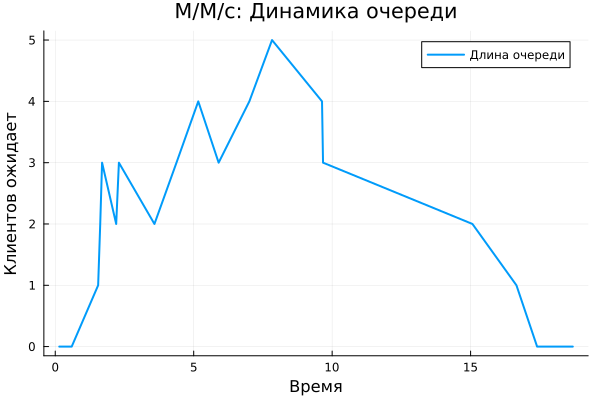
\includegraphics[width=0.7\textwidth,height=\textheight]{image/mmc_queue_length.png}

}

\caption{\label{fig-001}Динамика очереди}

\end{figure}%

Второй график, который я добавил, был графиком количества клиентов в
системе, из графика, аналогичного первому, мы можем видеть, что
наибольшее количество клиентов находится в пределах 5-10 единиц
времени(рис.5)

\begin{figure}

\centering{

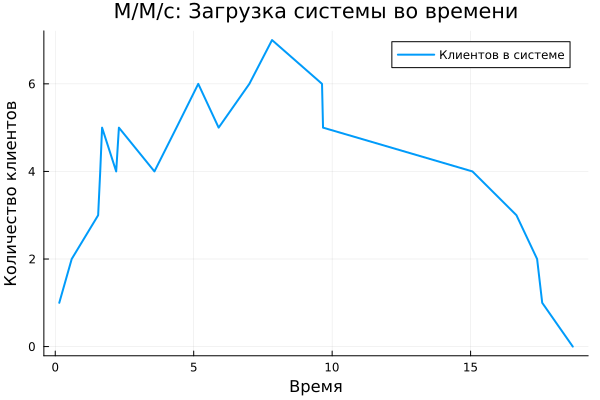
\includegraphics[width=0.7\textwidth,height=\textheight]{image/mmc_system_load.png}

}

\caption{\label{fig-001}Загрузка системы во времени}

\end{figure}%

Третий график предназначен для проверки того, насколько загружен сервер
по сравнению с теоретическим порогом (ρ), из графика мы видим, что
сервер загружен больше, чем ожидалось(рис.6)

\begin{figure}

\centering{

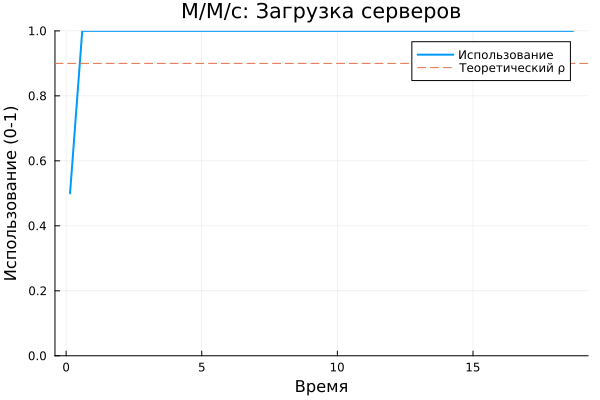
\includegraphics[width=0.7\textwidth,height=\textheight]{image/mmc_utilization.png}

}

\caption{\label{fig-001}Загрузка серверов}

\end{figure}%

\textbf{Ниже приведен код, результаты расчетов и графики для кода в
файле scripts/model\_mmc.qmd}

\chapter{Модель массового обслуживания
M/M/c}\label{ux43cux43eux434ux435ux43bux44c-ux43cux430ux441ux441ux43eux432ux43eux433ux43e-ux43eux431ux441ux43bux443ux436ux438ux432ux430ux43dux438ux44f-mmc}

Данная симуляция моделирует многоканальную систему массового
обслуживания с пуассоновским входящим потоком (интенсивность λ) и
экспоненциальным временем обслуживания (интенсивность μ). Клиенты
поступают, ожидают в очереди FIFO, если все серверы заняты, затем
обслуживаются и покидают систему.

\section{Загрузка необходимых
пакетов}\label{ux437ux430ux433ux440ux443ux437ux43aux430-ux43dux435ux43eux431ux445ux43eux434ux438ux43cux44bux445-ux43fux430ux43aux435ux442ux43eux432}

\begin{Shaded}
\begin{Highlighting}[]
\ImportTok{using} \BuiltInTok{DrWatson}
\PreprocessorTok{@quickactivate} \StringTok{"project"}

\ImportTok{using} \BuiltInTok{StableRNGs}
\ImportTok{using} \BuiltInTok{Distributions}
\ImportTok{using} \BuiltInTok{ConcurrentSim}
\ImportTok{using} \BuiltInTok{ResumableFunctions}
\ImportTok{using} \BuiltInTok{DataFrames}
\ImportTok{using} \BuiltInTok{Plots}
\ImportTok{using} \BuiltInTok{CSV}
\FunctionTok{gr}\NormalTok{(fmt}\OperatorTok{=:}\NormalTok{png)}
\end{Highlighting}
\end{Shaded}

\begin{verbatim}
┌ Warning: DrWatson could not find find a project file by recursively checking given `dir` and its parents. Returning `nothing` instead.
│ (given dir: /home/nelianjovu)
└ @ DrWatson ~/.julia/packages/DrWatson/2QF5p/src/project_setup.jl:84
\end{verbatim}

\begin{verbatim}
Plots.GRBackend()
\end{verbatim}

\section{Параметры
симуляции}\label{ux43fux430ux440ux430ux43cux435ux442ux440ux44b-ux441ux438ux43cux443ux43bux44fux446ux438ux438}

\begin{Shaded}
\begin{Highlighting}[]
\NormalTok{rng }\OperatorTok{=} \FunctionTok{StableRNG}\NormalTok{(}\FloatTok{123}\NormalTok{)}
\NormalTok{num\_customers }\OperatorTok{=} \FloatTok{10}
\NormalTok{num\_servers }\OperatorTok{=} \FloatTok{2}
\NormalTok{mu }\OperatorTok{=} \FloatTok{1.0} \OperatorTok{/} \FloatTok{2}
\NormalTok{lam }\OperatorTok{=} \FloatTok{0.9}
\NormalTok{arrival\_dist }\OperatorTok{=} \FunctionTok{Exponential}\NormalTok{(}\FloatTok{1} \OperatorTok{/}\NormalTok{ lam)}
\NormalTok{service\_dist }\OperatorTok{=} \FunctionTok{Exponential}\NormalTok{(}\FloatTok{1} \OperatorTok{/}\NormalTok{ mu)}
\end{Highlighting}
\end{Shaded}

\begin{verbatim}
Exponential{Float64}(θ=2.0)
\end{verbatim}

\section{Массивы для сбора
данных}\label{ux43cux430ux441ux441ux438ux432ux44b-ux434ux43bux44f-ux441ux431ux43eux440ux430-ux434ux430ux43dux43dux44bux445}

\begin{Shaded}
\begin{Highlighting}[]
\NormalTok{history }\OperatorTok{=} \FunctionTok{Vector}\DataTypeTok{\{Tuple\{Float64, String, Int\}\}}\NormalTok{()}
\end{Highlighting}
\end{Shaded}

\begin{verbatim}
Tuple{Float64, String, Int64}[]
\end{verbatim}

\section{Поведение
клиента}\label{ux43fux43eux432ux435ux434ux435ux43dux438ux435-ux43aux43bux438ux435ux43dux442ux430}

\begin{Shaded}
\begin{Highlighting}[]
\PreprocessorTok{@resumable} \KeywordTok{function} \FunctionTok{customer}\NormalTok{(}
\NormalTok{    env}\OperatorTok{::}\DataTypeTok{Environment}\NormalTok{,}
\NormalTok{    server}\OperatorTok{::}\DataTypeTok{Resource}\NormalTok{,}
\NormalTok{    id}\OperatorTok{::}\DataTypeTok{Integer}\NormalTok{,}
\NormalTok{    t\_a}\OperatorTok{::}\DataTypeTok{Float64}\NormalTok{,}
\NormalTok{    d\_s}\OperatorTok{::}\DataTypeTok{Distribution}\NormalTok{,}
\NormalTok{)}
    \PreprocessorTok{@yield} \FunctionTok{timeout}\NormalTok{(env, t\_a)}
    \FunctionTok{println}\NormalTok{(}\StringTok{"Customer }\SpecialCharTok{$}\NormalTok{id}\StringTok{ arrived: "}\NormalTok{, }\FunctionTok{now}\NormalTok{(env))}
    \FunctionTok{push!}\NormalTok{(history, (}\FunctionTok{now}\NormalTok{(env), }\StringTok{"arrived"}\NormalTok{, id))}

    \PreprocessorTok{@yield} \FunctionTok{request}\NormalTok{(server)}
    \FunctionTok{println}\NormalTok{(}\StringTok{"Customer }\SpecialCharTok{$}\NormalTok{id}\StringTok{ entered service: "}\NormalTok{, }\FunctionTok{now}\NormalTok{(env))}
    \FunctionTok{push!}\NormalTok{(history, (}\FunctionTok{now}\NormalTok{(env), }\StringTok{"started"}\NormalTok{, id))}

    \PreprocessorTok{@yield} \FunctionTok{timeout}\NormalTok{(env, }\FunctionTok{rand}\NormalTok{(rng, d\_s))}
    \PreprocessorTok{@yield} \FunctionTok{unlock}\NormalTok{(server)}
    \FunctionTok{println}\NormalTok{(}\StringTok{"Customer }\SpecialCharTok{$}\NormalTok{id}\StringTok{ exited service: "}\NormalTok{, }\FunctionTok{now}\NormalTok{(env))}
    \FunctionTok{push!}\NormalTok{(history, (}\FunctionTok{now}\NormalTok{(env), }\StringTok{"exited"}\NormalTok{, id))}
\KeywordTok{end}
\end{Highlighting}
\end{Shaded}

\begin{verbatim}
customer (generic function with 1 method)
\end{verbatim}

\section{Запуск
симуляции}\label{ux437ux430ux43fux443ux441ux43a-ux441ux438ux43cux443ux43bux44fux446ux438ux438}

\begin{Shaded}
\begin{Highlighting}[]
\KeywordTok{function} \FunctionTok{setup\_and\_run}\NormalTok{()}
\NormalTok{    sim }\OperatorTok{=} \FunctionTok{Simulation}\NormalTok{()}
\NormalTok{    server }\OperatorTok{=} \FunctionTok{Resource}\NormalTok{(sim, num\_servers)}
\NormalTok{    arrival\_time }\OperatorTok{=} \FloatTok{0.0}

    \ControlFlowTok{for}\NormalTok{ i }\OperatorTok{=} \FloatTok{1}\OperatorTok{:}\NormalTok{num\_customers}
\NormalTok{        arrival\_time }\OperatorTok{+=} \FunctionTok{rand}\NormalTok{(rng, arrival\_dist)}
        \PreprocessorTok{@process} \FunctionTok{customer}\NormalTok{(sim, server, i, arrival\_time, service\_dist)}
    \ControlFlowTok{end}

    \FunctionTok{run}\NormalTok{(sim)}
\KeywordTok{end}

\FunctionTok{setup\_and\_run}\NormalTok{()}
\end{Highlighting}
\end{Shaded}

\begin{verbatim}
Customer 1 arrived: 0.14518451436852475
Customer 1 entered service: 0.14518451436852475
Customer 2 arrived: 0.5941831542903504
Customer 2 entered service: 0.5941831542903504
Customer 3 arrived: 1.5490648267819074
Customer 4 arrived: 1.6242796925312217
Customer 5 arrived: 1.6911000709069648
Customer 1 exited service: 2.200985520126681
Customer 3 entered service: 2.200985520126681
Customer 6 arrived: 2.2989039524296317
Customer 3 exited service: 3.5822120399442174
Customer 4 entered service: 3.5822120399442174
Customer 7 arrived: 4.377930221620456
Customer 8 arrived: 5.16494279700802
Customer 2 exited service: 5.900722829377648
Customer 5 entered service: 5.900722829377648
Customer 9 arrived: 7.0099944106308705
Customer 10 arrived: 7.828990220943469
Customer 5 exited service: 9.634196437885254
Customer 6 entered service: 9.634196437885254
Customer 4 exited service: 9.670688398447817
Customer 7 entered service: 9.670688398447817
Customer 7 exited service: 15.066978111608014
Customer 8 entered service: 15.066978111608014
Customer 8 exited service: 16.655548432659554
Customer 9 entered service: 16.655548432659554
Customer 6 exited service: 17.401833154870328
Customer 10 entered service: 17.401833154870328
Customer 9 exited service: 17.586065352135993
Customer 10 exited service: 18.690264775280085
\end{verbatim}

\section{Постобработка: построение временных
рядов}\label{ux43fux43eux441ux442ux43eux431ux440ux430ux431ux43eux442ux43aux430-ux43fux43eux441ux442ux440ux43eux435ux43dux438ux435-ux432ux440ux435ux43cux435ux43dux43dux44bux445-ux440ux44fux434ux43eux432}

\begin{Shaded}
\begin{Highlighting}[]
\NormalTok{times }\OperatorTok{=} \FunctionTok{sort}\NormalTok{(}\FunctionTok{unique}\NormalTok{([t for (t, \_, \_) }\KeywordTok{in}\NormalTok{ history]))}
\NormalTok{system\_count }\OperatorTok{=} \FunctionTok{zeros}\NormalTok{(}\DataTypeTok{Int}\NormalTok{, }\FunctionTok{length}\NormalTok{(times))}
\NormalTok{queue\_count }\OperatorTok{=} \FunctionTok{zeros}\NormalTok{(}\DataTypeTok{Int}\NormalTok{, }\FunctionTok{length}\NormalTok{(times))}
\NormalTok{server\_usage }\OperatorTok{=} \FunctionTok{zeros}\NormalTok{(}\DataTypeTok{Float64}\NormalTok{, }\FunctionTok{length}\NormalTok{(times))}

\ControlFlowTok{for}\NormalTok{ (idx, t) }\KeywordTok{in} \FunctionTok{enumerate}\NormalTok{(times)}
\NormalTok{    arrived }\OperatorTok{=} \FunctionTok{count}\NormalTok{(x }\OperatorTok{{-}\textgreater{}}\NormalTok{ x[}\FloatTok{1}\NormalTok{] }\OperatorTok{\textless{}=}\NormalTok{ t }\OperatorTok{\&\&}\NormalTok{ x[}\FloatTok{2}\NormalTok{] }\OperatorTok{==} \StringTok{"arrived"}\NormalTok{, history)}
\NormalTok{    exited }\OperatorTok{=} \FunctionTok{count}\NormalTok{(x }\OperatorTok{{-}\textgreater{}}\NormalTok{ x[}\FloatTok{1}\NormalTok{] }\OperatorTok{\textless{}=}\NormalTok{ t }\OperatorTok{\&\&}\NormalTok{ x[}\FloatTok{2}\NormalTok{] }\OperatorTok{==} \StringTok{"exited"}\NormalTok{, history)}
\NormalTok{    started }\OperatorTok{=} \FunctionTok{count}\NormalTok{(x }\OperatorTok{{-}\textgreater{}}\NormalTok{ x[}\FloatTok{1}\NormalTok{] }\OperatorTok{\textless{}=}\NormalTok{ t }\OperatorTok{\&\&}\NormalTok{ x[}\FloatTok{2}\NormalTok{] }\OperatorTok{==} \StringTok{"started"}\NormalTok{, history)}

\NormalTok{    system\_count[idx] }\OperatorTok{=}\NormalTok{ arrived }\OperatorTok{{-}}\NormalTok{ exited}
\NormalTok{    queue\_count[idx] }\OperatorTok{=}\NormalTok{ arrived }\OperatorTok{{-}}\NormalTok{ started}
\NormalTok{    server\_usage[idx] }\OperatorTok{=} \FunctionTok{min}\NormalTok{(}\FloatTok{1.0}\NormalTok{, started }\OperatorTok{/}\NormalTok{ num\_servers)}
\ControlFlowTok{end}
\end{Highlighting}
\end{Shaded}

\section{Создание DataFrame с
результатами}\label{ux441ux43eux437ux434ux430ux43dux438ux435-dataframe-ux441-ux440ux435ux437ux443ux43bux44cux442ux430ux442ux430ux43cux438}

\begin{Shaded}
\begin{Highlighting}[]
\NormalTok{df\_results }\OperatorTok{=} \FunctionTok{DataFrame}\NormalTok{(}
\NormalTok{    time }\OperatorTok{=}\NormalTok{ times,}
\NormalTok{    n\_in\_system }\OperatorTok{=}\NormalTok{ system\_count,}
\NormalTok{    queue\_length }\OperatorTok{=}\NormalTok{ queue\_count,}
\NormalTok{    utilization }\OperatorTok{=}\NormalTok{ server\_usage}
\NormalTok{)}
\end{Highlighting}
\end{Shaded}

\begin{tabular}{r|cccc}
    & time & n\_in\_system & queue\_length & utilization\\
    \hline
    & Float64 & Int64 & Int64 & Float64\\
    \hline
    1 & 0.145185 & 1 & 0 & 0.5 \\
    2 & 0.594183 & 2 & 0 & 1.0 \\
    3 & 1.54906 & 3 & 1 & 1.0 \\
    4 & 1.62428 & 4 & 2 & 1.0 \\
    5 & 1.6911 & 5 & 3 & 1.0 \\
    6 & 2.20099 & 4 & 2 & 1.0 \\
    7 & 2.2989 & 5 & 3 & 1.0 \\
    8 & 3.58221 & 4 & 2 & 1.0 \\
    9 & 4.37793 & 5 & 3 & 1.0 \\
    10 & 5.16494 & 6 & 4 & 1.0 \\
    11 & 5.90072 & 5 & 3 & 1.0 \\
    12 & 7.00999 & 6 & 4 & 1.0 \\
    13 & 7.82899 & 7 & 5 & 1.0 \\
    14 & 9.6342 & 6 & 4 & 1.0 \\
    15 & 9.67069 & 5 & 3 & 1.0 \\
    16 & 15.067 & 4 & 2 & 1.0 \\
    17 & 16.6555 & 3 & 1 & 1.0 \\
    18 & 17.4018 & 2 & 0 & 1.0 \\
    19 & 17.5861 & 1 & 0 & 1.0 \\
    20 & 18.6903 & 0 & 0 & 1.0 \\
\end{tabular}

\section{Сохранение
данных}\label{ux441ux43eux445ux440ux430ux43dux435ux43dux438ux435-ux434ux430ux43dux43dux44bux445}

\begin{Shaded}
\begin{Highlighting}[]
\FunctionTok{mkpath}\NormalTok{(}\FunctionTok{datadir}\NormalTok{())}
\FunctionTok{mkpath}\NormalTok{(}\FunctionTok{plotsdir}\NormalTok{())}
\NormalTok{CSV.}\FunctionTok{write}\NormalTok{(}\FunctionTok{datadir}\NormalTok{(}\StringTok{"mmc\_results.csv"}\NormalTok{), df\_results)}
\end{Highlighting}
\end{Shaded}

\begin{verbatim}
"/home/nelianjovu/work/study/2026-1/2026-1==study--simulationmod/2026-1--study--simulationmod/labs/lab07/project/data/mmc_results.csv"
\end{verbatim}

\section{График 1: Количество клиентов в
системе}\label{ux433ux440ux430ux444ux438ux43a-1-ux43aux43eux43bux438ux447ux435ux441ux442ux432ux43e-ux43aux43bux438ux435ux43dux442ux43eux432-ux432-ux441ux438ux441ux442ux435ux43cux435}

\begin{Shaded}
\begin{Highlighting}[]
\NormalTok{p1 }\OperatorTok{=} \FunctionTok{plot}\NormalTok{(df\_results.time, df\_results.n\_in\_system,}
\NormalTok{    label }\OperatorTok{=} \StringTok{"Клиентов в системе"}\NormalTok{,}
\NormalTok{    xlabel }\OperatorTok{=} \StringTok{"Время"}\NormalTok{,}
\NormalTok{    ylabel }\OperatorTok{=} \StringTok{"Количество клиентов"}\NormalTok{,}
\NormalTok{    title }\OperatorTok{=} \StringTok{"M/M/c: Загрузка системы во времени"}\NormalTok{,}
\NormalTok{    linewidth }\OperatorTok{=} \FloatTok{2}\NormalTok{,}
\NormalTok{    legend }\OperatorTok{=} \OperatorTok{:}\NormalTok{topright)}
\FunctionTok{display}\NormalTok{(p1)}
\FunctionTok{savefig}\NormalTok{(}\FunctionTok{plotsdir}\NormalTok{(}\StringTok{"mmc\_system\_load.png"}\NormalTok{))}
\end{Highlighting}
\end{Shaded}

\includesvg{simmod-lab07-report (Нджову Нелиа)_files/figure-pdf/cell-11-output-1.svg}

\begin{verbatim}
"/home/nelianjovu/work/study/2026-1/2026-1==study--simulationmod/2026-1--study--simulationmod/labs/lab07/project/plots/mmc_system_load.png"
\end{verbatim}

\section{График 2: Длина очереди во
времени}\label{ux433ux440ux430ux444ux438ux43a-2-ux434ux43bux438ux43dux430-ux43eux447ux435ux440ux435ux434ux438-ux432ux43e-ux432ux440ux435ux43cux435ux43dux438}

\begin{Shaded}
\begin{Highlighting}[]
\NormalTok{p2 }\OperatorTok{=} \FunctionTok{plot}\NormalTok{(df\_results.time, df\_results.queue\_length,}
\NormalTok{    label }\OperatorTok{=} \StringTok{"Длина очереди"}\NormalTok{,}
\NormalTok{    xlabel }\OperatorTok{=} \StringTok{"Время"}\NormalTok{,}
\NormalTok{    ylabel }\OperatorTok{=} \StringTok{"Клиентов ожидает"}\NormalTok{,}
\NormalTok{    title }\OperatorTok{=} \StringTok{"M/M/c: Динамика очереди"}\NormalTok{,}
\NormalTok{    linewidth }\OperatorTok{=} \FloatTok{2}\NormalTok{,}
\NormalTok{    legend }\OperatorTok{=} \OperatorTok{:}\NormalTok{topright)}
\FunctionTok{display}\NormalTok{(p2)}
\FunctionTok{savefig}\NormalTok{(}\FunctionTok{plotsdir}\NormalTok{(}\StringTok{"mmc\_queue\_length.png"}\NormalTok{))}
\end{Highlighting}
\end{Shaded}

\includesvg{simmod-lab07-report (Нджову Нелиа)_files/figure-pdf/cell-12-output-1.svg}

\begin{verbatim}
"/home/nelianjovu/work/study/2026-1/2026-1==study--simulationmod/2026-1--study--simulationmod/labs/lab07/project/plots/mmc_queue_length.png"
\end{verbatim}

\section{График 3: Использование серверов во
времени}\label{ux433ux440ux430ux444ux438ux43a-3-ux438ux441ux43fux43eux43bux44cux437ux43eux432ux430ux43dux438ux435-ux441ux435ux440ux432ux435ux440ux43eux432-ux432ux43e-ux432ux440ux435ux43cux435ux43dux438}

\begin{Shaded}
\begin{Highlighting}[]
\NormalTok{ρ }\OperatorTok{=}\NormalTok{ lam }\OperatorTok{/}\NormalTok{ (num\_servers }\OperatorTok{*}\NormalTok{ mu)}
\NormalTok{p3 }\OperatorTok{=} \FunctionTok{plot}\NormalTok{(df\_results.time, df\_results.utilization,}
\NormalTok{    label }\OperatorTok{=} \StringTok{"Использование"}\NormalTok{,}
\NormalTok{    xlabel }\OperatorTok{=} \StringTok{"Время"}\NormalTok{,}
\NormalTok{    ylabel }\OperatorTok{=} \StringTok{"Использование (0{-}1)"}\NormalTok{,}
\NormalTok{    title }\OperatorTok{=} \StringTok{"M/M/c: Загрузка серверов"}\NormalTok{,}
\NormalTok{    linewidth }\OperatorTok{=} \FloatTok{2}\NormalTok{,}
\NormalTok{    legend }\OperatorTok{=} \OperatorTok{:}\NormalTok{topright,}
\NormalTok{    ylims }\OperatorTok{=}\NormalTok{ (}\FloatTok{0}\NormalTok{, }\FloatTok{1}\NormalTok{))}
\FunctionTok{hline!}\NormalTok{([ρ], label }\OperatorTok{=} \StringTok{"Теоретический ρ"}\NormalTok{, linestyle }\OperatorTok{=} \OperatorTok{:}\NormalTok{dash)}
\FunctionTok{display}\NormalTok{(p3)}
\FunctionTok{savefig}\NormalTok{(}\FunctionTok{plotsdir}\NormalTok{(}\StringTok{"mmc\_utilization.png"}\NormalTok{))}
\end{Highlighting}
\end{Shaded}

\includesvg{simmod-lab07-report (Нджову Нелиа)_files/figure-pdf/cell-13-output-1.svg}

\begin{verbatim}
"/home/nelianjovu/work/study/2026-1/2026-1==study--simulationmod/2026-1--study--simulationmod/labs/lab07/project/plots/mmc_utilization.png"
\end{verbatim}

\section{2. Модель
Росса}\label{ux43cux43eux434ux435ux43bux44c-ux440ux43eux441ux441ux430}

Я создала файл scripts/model\_mmc.jl и скопировала заданный скрипт в
него. Скрипт реализует систему ремонта машины с использованием запасных
частей из учебника Росса. Если машина выходит из строя, она немедленно
заменяется на запасную, а неисправная машина ремонтируется мастером,
если запасная машина недоступна, система выходит из строя. Я запускала
код и все сработала хорошо(рис.7).

\begin{figure}

\centering{


\includegraphics[width=0.7\textwidth,height=\textheight]{image/pic10.png}

}

\caption{\label{fig-001}Заданный скрипт}

\end{figure}%

После этого я перевожу код в структуру DrWatson и добавляю несколько
ремонтников(рис.8)

\begin{figure}

\centering{


\includegraphics[width=0.7\textwidth,height=\textheight]{image/pic6.png}

}

\caption{\label{fig-001}Добавление нескольких ремонтников}

\end{figure}%

Я экспериментирую с системой, используя разное количество машин(рис.9)

\begin{figure}

\centering{


\includegraphics[width=0.7\textwidth,height=\textheight]{image/pic7.png}

}

\caption{\label{fig-001}Разные конфигурации}

\end{figure}%

Затем я добавляю необходимую визуализацию(рис.10)

\begin{figure}

\centering{


\includegraphics[width=0.7\textwidth,height=\textheight]{image/pic11.png}

}

\caption{\label{fig-001}Визуализация}

\end{figure}%

На первом из которых показано количество работающих машин, запасных,
ремонтируемых машин и необходимых ремонтников(рис.11)

\begin{figure}

\centering{

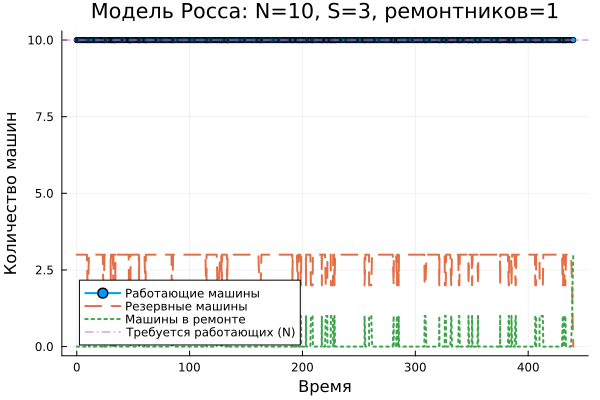
\includegraphics[width=0.7\textwidth,height=\textheight]{image/ross_dynamics_base.png}

}

\caption{\label{fig-001}Модель Росса}

\end{figure}%

Из второго графика видно, что количество ремонтников влияет на среднее
время простоя. Чем больше число ремонтников, тем больше времени
требуется системе для выхода из строя(рис.12)

\begin{figure}

\centering{

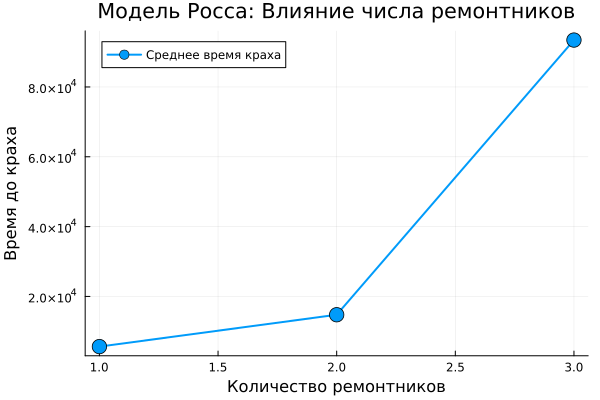
\includegraphics[width=0.7\textwidth,height=\textheight]{image/ross_repairmen_impact.png}

}

\caption{\label{fig-001}Модель Росса: Влияние числа ремонтников}

\end{figure}%

На третьем графике показано, как количество работающих машин влияет на
среднее время сбоя: чем больше количество работающих машин, тем больше
времени требуется системе для выхода из строя(рис.13)

\begin{figure}

\centering{

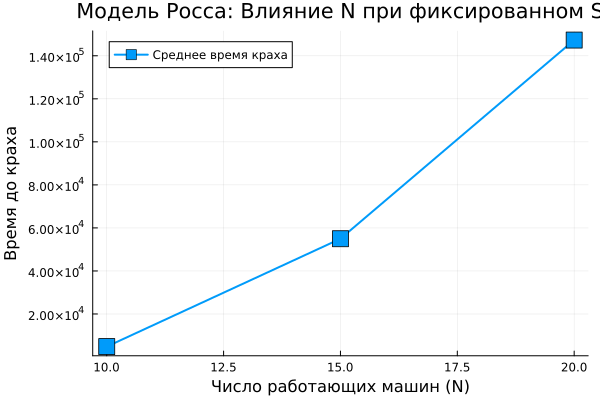
\includegraphics[width=0.7\textwidth,height=\textheight]{image/ross_config_comparison.png}

}

\caption{\label{fig-001}Модель Росса: Влияние N при фиксированном S}

\end{figure}%

Когда я сравнила результаты с аналитическим методом, выяснилось, что при
моделировании сбой происходит гораздо дольше, чем при
аналитическом(рис.14)

\begin{figure}

\centering{


\includegraphics[width=0.7\textwidth,height=\textheight]{image/pic8.png}

}

\caption{\label{fig-001}Сравнение с аналитическим методом}

\end{figure}%

\textbf{Ниже приведен код, результаты расчетов и графики для кода в
файле scripts/model\_ross.qmd}

\chapter{Модель Росса (Система с резервированием и
ремонтом)}\label{ux43cux43eux434ux435ux43bux44c-ux440ux43eux441ux441ux430-ux441ux438ux441ux442ux435ux43cux430-ux441-ux440ux435ux437ux435ux440ux432ux438ux440ux43eux432ux430ux43dux438ux435ux43c-ux438-ux440ux435ux43cux43eux43dux442ux43eux43c}

В системе находятся N работающих машин и S резервных. При поломке машина
заменяется резервной (если есть) и отправляется в ремонт. Если резерва
нет --- система падает. Ремонт выполняют несколько ремонтников.

\section{Загрузка необходимых
пакетов}\label{ux437ux430ux433ux440ux443ux437ux43aux430-ux43dux435ux43eux431ux445ux43eux434ux438ux43cux44bux445-ux43fux430ux43aux435ux442ux43eux432-1}

\begin{Shaded}
\begin{Highlighting}[]
\ImportTok{using} \BuiltInTok{DrWatson}
\PreprocessorTok{@quickactivate} \StringTok{"project"}

\ImportTok{using} \BuiltInTok{ResumableFunctions}
\ImportTok{using} \BuiltInTok{ConcurrentSim}
\ImportTok{using} \BuiltInTok{Distributions}
\ImportTok{using} \BuiltInTok{Random}
\ImportTok{using} \BuiltInTok{StableRNGs}
\ImportTok{using} \BuiltInTok{DataFrames}
\ImportTok{using} \BuiltInTok{CSV}
\ImportTok{using} \BuiltInTok{Plots}
\ImportTok{using} \BuiltInTok{Statistics}
\FunctionTok{gr}\NormalTok{(fmt}\OperatorTok{=:}\NormalTok{png)}
\end{Highlighting}
\end{Shaded}

\begin{verbatim}
┌ Warning: DrWatson could not find find a project file by recursively checking given `dir` and its parents. Returning `nothing` instead.
│ (given dir: /home/nelianjovu)
└ @ DrWatson ~/.julia/packages/DrWatson/2QF5p/src/project_setup.jl:84
\end{verbatim}

\begin{verbatim}
Plots.GRBackend()
\end{verbatim}

\section{Параметры
симуляции}\label{ux43fux430ux440ux430ux43cux435ux442ux440ux44b-ux441ux438ux43cux443ux43bux44fux446ux438ux438-1}

\begin{Shaded}
\begin{Highlighting}[]
\KeywordTok{const}\NormalTok{ RUNS }\OperatorTok{=} \FloatTok{5}
\KeywordTok{const}\NormalTok{ N }\OperatorTok{=} \FloatTok{10}
\KeywordTok{const}\NormalTok{ S }\OperatorTok{=} \FloatTok{3}
\KeywordTok{const}\NormalTok{ LAMBDA }\OperatorTok{=} \FloatTok{100.0}
\KeywordTok{const}\NormalTok{ MU }\OperatorTok{=} \FloatTok{1.0}
\KeywordTok{const}\NormalTok{ SEED }\OperatorTok{=} \FloatTok{42}

\NormalTok{rng }\OperatorTok{=} \FunctionTok{StableRNG}\NormalTok{(SEED)}
\NormalTok{F }\OperatorTok{=} \FunctionTok{Exponential}\NormalTok{(LAMBDA)}
\NormalTok{G }\OperatorTok{=} \FunctionTok{Exponential}\NormalTok{(}\FloatTok{1}\OperatorTok{/}\NormalTok{MU)}
\end{Highlighting}
\end{Shaded}

\begin{verbatim}
Exponential{Float64}(θ=1.0)
\end{verbatim}

\section{Структура для хранения состояния
системы}\label{ux441ux442ux440ux443ux43aux442ux443ux440ux430-ux434ux43bux44f-ux445ux440ux430ux43dux435ux43dux438ux44f-ux441ux43eux441ux442ux43eux44fux43dux438ux44f-ux441ux438ux441ux442ux435ux43cux44b}

\begin{Shaded}
\begin{Highlighting}[]
\KeywordTok{mutable struct}\NormalTok{ SystemState}
\NormalTok{    operational}\OperatorTok{::}\DataTypeTok{Int}
\NormalTok{    in\_repair}\OperatorTok{::}\DataTypeTok{Int}
\NormalTok{    spares}\OperatorTok{::}\DataTypeTok{Int}
\NormalTok{    history}\OperatorTok{::}\DataTypeTok{Vector\{Tuple\{Float64, Int, Int, Int\}\}}
\KeywordTok{end}
\end{Highlighting}
\end{Shaded}

\section{Поведение
машины}\label{ux43fux43eux432ux435ux434ux435ux43dux438ux435-ux43cux430ux448ux438ux43dux44b}

\begin{Shaded}
\begin{Highlighting}[]
\PreprocessorTok{@resumable} \KeywordTok{function} \FunctionTok{machine}\NormalTok{(}
\NormalTok{    env}\OperatorTok{::}\DataTypeTok{Environment}\NormalTok{,}
\NormalTok{    repair\_queue}\OperatorTok{::}\DataTypeTok{Resource}\NormalTok{,}
\NormalTok{    state}\OperatorTok{::}\DataTypeTok{SystemState}\NormalTok{,}
\NormalTok{    machine\_id}\OperatorTok{::}\DataTypeTok{Int}\NormalTok{,}
\NormalTok{)}
    \ControlFlowTok{while} \ConstantTok{true}
        \PreprocessorTok{@yield} \FunctionTok{timeout}\NormalTok{(env, }\FunctionTok{rand}\NormalTok{(rng, F))}

        \ControlFlowTok{if}\NormalTok{ state.operational }\OperatorTok{\textgreater{}} \FloatTok{0}
\NormalTok{            state.operational }\OperatorTok{{-}=} \FloatTok{1}
        \ControlFlowTok{end}

        \ControlFlowTok{if}\NormalTok{ state.spares }\OperatorTok{\textgreater{}} \FloatTok{0}
\NormalTok{            state.spares }\OperatorTok{{-}=} \FloatTok{1}
\NormalTok{            state.operational }\OperatorTok{+=} \FloatTok{1}
        \ControlFlowTok{else}
            \FunctionTok{throw}\NormalTok{(}\FunctionTok{StopSimulation}\NormalTok{(}\StringTok{"No more spares!"}\NormalTok{))}
        \ControlFlowTok{end}

        \FunctionTok{push!}\NormalTok{(state.history, (}\FunctionTok{now}\NormalTok{(env), state.operational, state.in\_repair, state.spares))}

\NormalTok{        state.in\_repair }\OperatorTok{+=} \FloatTok{1}
        \FunctionTok{push!}\NormalTok{(state.history, (}\FunctionTok{now}\NormalTok{(env), state.operational, state.in\_repair, state.spares))}

        \PreprocessorTok{@yield} \FunctionTok{request}\NormalTok{(repair\_queue)}
        \PreprocessorTok{@yield} \FunctionTok{timeout}\NormalTok{(env, }\FunctionTok{rand}\NormalTok{(rng, G))}
        \PreprocessorTok{@yield} \FunctionTok{unlock}\NormalTok{(repair\_queue)}

\NormalTok{        state.in\_repair }\OperatorTok{{-}=} \FloatTok{1}
\NormalTok{        state.spares }\OperatorTok{+=} \FloatTok{1}
        \FunctionTok{push!}\NormalTok{(state.history, (}\FunctionTok{now}\NormalTok{(env), state.operational, state.in\_repair, state.spares))}
    \ControlFlowTok{end}
\KeywordTok{end}
\end{Highlighting}
\end{Shaded}

\begin{verbatim}
machine (generic function with 1 method)
\end{verbatim}

\section{Запуск
симуляции}\label{ux437ux430ux43fux443ux441ux43a-ux441ux438ux43cux443ux43bux44fux446ux438ux438-1}

\begin{Shaded}
\begin{Highlighting}[]
\KeywordTok{function} \FunctionTok{sim\_repair}\NormalTok{(N}\OperatorTok{::}\DataTypeTok{Int}\NormalTok{, S}\OperatorTok{::}\DataTypeTok{Int}\NormalTok{, num\_repairmen}\OperatorTok{::}\DataTypeTok{Int}\NormalTok{)}
\NormalTok{    sim }\OperatorTok{=} \FunctionTok{Simulation}\NormalTok{()}
\NormalTok{    repair\_queue }\OperatorTok{=} \FunctionTok{Resource}\NormalTok{(sim, num\_repairmen)}

\NormalTok{    state }\OperatorTok{=} \FunctionTok{SystemState}\NormalTok{(N, }\FloatTok{0}\NormalTok{, S, }\FunctionTok{Vector}\DataTypeTok{\{Tuple\{Float64, Int, Int, Int\}\}}\NormalTok{())}
    \FunctionTok{push!}\NormalTok{(state.history, (}\FloatTok{0.0}\NormalTok{, N, }\FloatTok{0}\NormalTok{, S))}

    \ControlFlowTok{for}\NormalTok{ i }\KeywordTok{in} \FloatTok{1}\OperatorTok{:}\NormalTok{N}
        \PreprocessorTok{@process} \FunctionTok{machine}\NormalTok{(sim, repair\_queue, state, i)}
    \ControlFlowTok{end}

    \ControlFlowTok{for}\NormalTok{ i }\KeywordTok{in} \FloatTok{1}\OperatorTok{:}\NormalTok{S}
        \PreprocessorTok{@process} \FunctionTok{machine}\NormalTok{(sim, repair\_queue, state, N }\OperatorTok{+}\NormalTok{ i)}
    \ControlFlowTok{end}

\NormalTok{    try}
        \FunctionTok{run}\NormalTok{(sim)}
        \ControlFlowTok{return} \FunctionTok{now}\NormalTok{(sim), state.history}
\NormalTok{    catch }\ConstantTok{e}
        \ControlFlowTok{if} \FunctionTok{isa}\NormalTok{(}\ConstantTok{e}\NormalTok{, StopSimulation)}
\NormalTok{            msg }\OperatorTok{=} \ConstantTok{e}\NormalTok{.msg}
\NormalTok{            stop\_time }\OperatorTok{=} \FunctionTok{now}\NormalTok{(sim)}
            \FunctionTok{println}\NormalTok{(}\StringTok{"At time }\SpecialCharTok{$}\NormalTok{stop\_time}\StringTok{: }\SpecialCharTok{$}\NormalTok{msg}\StringTok{"}\NormalTok{)}
            \ControlFlowTok{return}\NormalTok{ stop\_time, state.history}
        \ControlFlowTok{else}
            \FunctionTok{rethrow}\NormalTok{()}
        \ControlFlowTok{end}
    \KeywordTok{end}
\KeywordTok{end}
\end{Highlighting}
\end{Shaded}

\begin{verbatim}
sim_repair (generic function with 1 method)
\end{verbatim}

\section{Построение DataFrame из
истории}\label{ux43fux43eux441ux442ux440ux43eux435ux43dux438ux435-dataframe-ux438ux437-ux438ux441ux442ux43eux440ux438ux438}

\begin{Shaded}
\begin{Highlighting}[]
\KeywordTok{function} \FunctionTok{history\_to\_dataframe}\NormalTok{(history}\OperatorTok{::}\DataTypeTok{Vector\{Tuple\{Float64, Int, Int, Int\}\}}\NormalTok{)}
\NormalTok{    times }\OperatorTok{=}\NormalTok{ [t for (t, \_, \_, \_) }\KeywordTok{in}\NormalTok{ history]}
\NormalTok{    operational }\OperatorTok{=}\NormalTok{ [op for (\_, op, \_, \_) }\KeywordTok{in}\NormalTok{ history]}
\NormalTok{    in\_repair }\OperatorTok{=}\NormalTok{ [rep for (\_, \_, rep, \_) }\KeywordTok{in}\NormalTok{ history]}
\NormalTok{    spares }\OperatorTok{=}\NormalTok{ [sp for (\_, \_, \_, sp) }\KeywordTok{in}\NormalTok{ history]}

\NormalTok{    all\_times }\OperatorTok{=} \FunctionTok{sort}\NormalTok{(}\FunctionTok{unique}\NormalTok{(}\FunctionTok{vcat}\NormalTok{(times, }\FloatTok{0.0}\OperatorTok{:}\FloatTok{1.0}\OperatorTok{:}\FunctionTok{maximum}\NormalTok{(times))))}
\NormalTok{    op\_continuous }\OperatorTok{=} \FunctionTok{zeros}\NormalTok{(}\DataTypeTok{Int}\NormalTok{, }\FunctionTok{length}\NormalTok{(all\_times))}
\NormalTok{    rep\_continuous }\OperatorTok{=} \FunctionTok{zeros}\NormalTok{(}\DataTypeTok{Int}\NormalTok{, }\FunctionTok{length}\NormalTok{(all\_times))}
\NormalTok{    spare\_continuous }\OperatorTok{=} \FunctionTok{zeros}\NormalTok{(}\DataTypeTok{Int}\NormalTok{, }\FunctionTok{length}\NormalTok{(all\_times))}

    \ControlFlowTok{for}\NormalTok{ (idx, t) }\KeywordTok{in} \FunctionTok{enumerate}\NormalTok{(all\_times)}
\NormalTok{        last\_idx }\OperatorTok{=} \FunctionTok{findlast}\NormalTok{(ti }\OperatorTok{{-}\textgreater{}}\NormalTok{ ti }\OperatorTok{\textless{}=}\NormalTok{ t, times)}
        \ControlFlowTok{if}\NormalTok{ last\_idx }\OperatorTok{!==} \ConstantTok{nothing}
\NormalTok{            op\_continuous[idx] }\OperatorTok{=}\NormalTok{ operational[last\_idx]}
\NormalTok{            rep\_continuous[idx] }\OperatorTok{=}\NormalTok{ in\_repair[last\_idx]}
\NormalTok{            spare\_continuous[idx] }\OperatorTok{=}\NormalTok{ spares[last\_idx]}
        \ControlFlowTok{elseif}\NormalTok{ idx }\OperatorTok{\textgreater{}} \FloatTok{1}
\NormalTok{            op\_continuous[idx] }\OperatorTok{=}\NormalTok{ op\_continuous[idx}\OperatorTok{{-}}\FloatTok{1}\NormalTok{]}
\NormalTok{            rep\_continuous[idx] }\OperatorTok{=}\NormalTok{ rep\_continuous[idx}\OperatorTok{{-}}\FloatTok{1}\NormalTok{]}
\NormalTok{            spare\_continuous[idx] }\OperatorTok{=}\NormalTok{ spare\_continuous[idx}\OperatorTok{{-}}\FloatTok{1}\NormalTok{]}
        \ControlFlowTok{end}
    \ControlFlowTok{end}

    \ControlFlowTok{return} \FunctionTok{DataFrame}\NormalTok{(}
\NormalTok{        time }\OperatorTok{=}\NormalTok{ all\_times,}
\NormalTok{        operational }\OperatorTok{=}\NormalTok{ op\_continuous,}
\NormalTok{        in\_repair }\OperatorTok{=}\NormalTok{ rep\_continuous,}
\NormalTok{        spares }\OperatorTok{=}\NormalTok{ spare\_continuous}
\NormalTok{    )}
\KeywordTok{end}
\end{Highlighting}
\end{Shaded}

\begin{verbatim}
history_to_dataframe (generic function with 1 method)
\end{verbatim}

\section{Создание
каталогов}\label{ux441ux43eux437ux434ux430ux43dux438ux435-ux43aux430ux442ux430ux43bux43eux433ux43eux432}

\begin{Shaded}
\begin{Highlighting}[]
\FunctionTok{mkpath}\NormalTok{(}\FunctionTok{datadir}\NormalTok{())}
\FunctionTok{mkpath}\NormalTok{(}\FunctionTok{plotsdir}\NormalTok{())}
\end{Highlighting}
\end{Shaded}

\begin{verbatim}
"/home/nelianjovu/work/study/2026-1/2026-1==study--simulationmod/2026-1--study--simulationmod/labs/lab07/project/plots"
\end{verbatim}

\section{Эксперимент 1: Базовый прогон (как в
оригинале)}\label{ux44dux43aux441ux43fux435ux440ux438ux43cux435ux43dux442-1-ux431ux430ux437ux43eux432ux44bux439-ux43fux440ux43eux433ux43eux43d-ux43aux430ux43a-ux432-ux43eux440ux438ux433ux438ux43dux430ux43bux435}

\begin{Shaded}
\begin{Highlighting}[]
\NormalTok{results\_base }\OperatorTok{=} \DataTypeTok{Float64}\NormalTok{[]}

\ControlFlowTok{for}\NormalTok{ i }\KeywordTok{in} \FloatTok{1}\OperatorTok{:}\NormalTok{RUNS}
\NormalTok{    crash\_time, \_ }\OperatorTok{=} \FunctionTok{sim\_repair}\NormalTok{(N, S, }\FloatTok{1}\NormalTok{)}
    \FunctionTok{push!}\NormalTok{(results\_base, crash\_time)}
\ControlFlowTok{end}

\NormalTok{avg\_crash\_base }\OperatorTok{=} \FunctionTok{sum}\NormalTok{(results\_base) }\OperatorTok{/}\NormalTok{ RUNS}
\FunctionTok{println}\NormalTok{(}\StringTok{"}\SpecialCharTok{\textbackslash{}n}\StringTok{Average crash time: }\SpecialCharTok{$}\NormalTok{avg\_crash\_base}\StringTok{"}\NormalTok{)}
\end{Highlighting}
\end{Shaded}

\begin{verbatim}

Average crash time: 15345.935446105408
\end{verbatim}

\section{График 1: Динамика исправных машин (базовый
прогон)}\label{ux433ux440ux430ux444ux438ux43a-1-ux434ux438ux43dux430ux43cux438ux43aux430-ux438ux441ux43fux440ux430ux432ux43dux44bux445-ux43cux430ux448ux438ux43d-ux431ux430ux437ux43eux432ux44bux439-ux43fux440ux43eux433ux43eux43d}

\begin{Shaded}
\begin{Highlighting}[]
\NormalTok{\_, history\_base }\OperatorTok{=} \FunctionTok{sim\_repair}\NormalTok{(N, S, }\FloatTok{1}\NormalTok{)}
\NormalTok{df\_dynamics\_base }\OperatorTok{=} \FunctionTok{history\_to\_dataframe}\NormalTok{(history\_base)}

\NormalTok{p1 }\OperatorTok{=} \FunctionTok{plot}\NormalTok{(df\_dynamics\_base.time, df\_dynamics\_base.operational,}
\NormalTok{    marker }\OperatorTok{=} \OperatorTok{:}\NormalTok{circle, markersize }\OperatorTok{=} \FloatTok{3}\NormalTok{, linewidth }\OperatorTok{=} \FloatTok{2}\NormalTok{,}
\NormalTok{    label }\OperatorTok{=} \StringTok{"Работающие машины"}\NormalTok{,}
\NormalTok{    xlabel }\OperatorTok{=} \StringTok{"Время"}\NormalTok{, ylabel }\OperatorTok{=} \StringTok{"Количество машин"}\NormalTok{,}
\NormalTok{    title }\OperatorTok{=} \StringTok{"Модель Росса: N=}\SpecialCharTok{$}\NormalTok{N}\StringTok{, S=}\SpecialCharTok{$}\NormalTok{S}\StringTok{, ремонтников=1"}\NormalTok{)}
\FunctionTok{plot!}\NormalTok{(p1, df\_dynamics\_base.time, df\_dynamics\_base.spares,}
\NormalTok{    label }\OperatorTok{=} \StringTok{"Резервные машины"}\NormalTok{, linewidth }\OperatorTok{=} \FloatTok{2}\NormalTok{, linestyle }\OperatorTok{=} \OperatorTok{:}\NormalTok{dash)}
\FunctionTok{plot!}\NormalTok{(p1, df\_dynamics\_base.time, df\_dynamics\_base.in\_repair,}
\NormalTok{    label }\OperatorTok{=} \StringTok{"Машины в ремонте"}\NormalTok{, linewidth }\OperatorTok{=} \FloatTok{2}\NormalTok{, linestyle }\OperatorTok{=} \OperatorTok{:}\NormalTok{dot)}
\FunctionTok{hline!}\NormalTok{([N], label }\OperatorTok{=} \StringTok{"Требуется работающих (N)"}\NormalTok{, linestyle }\OperatorTok{=} \OperatorTok{:}\NormalTok{dashdot)}
\FunctionTok{savefig}\NormalTok{(}\FunctionTok{plotsdir}\NormalTok{(}\StringTok{"ross\_dynamics\_base.png"}\NormalTok{))}
\end{Highlighting}
\end{Shaded}

\begin{verbatim}
"/home/nelianjovu/work/study/2026-1/2026-1==study--simulationmod/2026-1--study--simulationmod/labs/lab07/project/plots/ross_dynamics_base.png"
\end{verbatim}

\section{Эксперимент 2: Разное количество
ремонтников}\label{ux44dux43aux441ux43fux435ux440ux438ux43cux435ux43dux442-2-ux440ux430ux437ux43dux43eux435-ux43aux43eux43bux438ux447ux435ux441ux442ux432ux43e-ux440ux435ux43cux43eux43dux442ux43dux438ux43aux43eux432}

\begin{Shaded}
\begin{Highlighting}[]
\FunctionTok{println}\NormalTok{(}\StringTok{"ЭКСПЕРИМЕНТ 1: Влияние количества ремонтников"}\NormalTok{)}

\NormalTok{num\_repairmen\_list }\OperatorTok{=}\NormalTok{ [}\FloatTok{1}\NormalTok{, }\FloatTok{2}\NormalTok{, }\FloatTok{3}\NormalTok{]}
\NormalTok{results\_repairmen }\OperatorTok{=}\NormalTok{ []}

\ControlFlowTok{for}\NormalTok{ num\_rep }\KeywordTok{in}\NormalTok{ num\_repairmen\_list}
    \FunctionTok{println}\NormalTok{(}\StringTok{"}\SpecialCharTok{\textbackslash{}n}\StringTok{Ремонтников: }\SpecialCharTok{$}\NormalTok{num\_rep}\StringTok{"}\NormalTok{)}
\NormalTok{    crash\_times }\OperatorTok{=} \DataTypeTok{Float64}\NormalTok{[]}
    \ControlFlowTok{for}\NormalTok{ run }\KeywordTok{in} \FloatTok{1}\OperatorTok{:}\NormalTok{RUNS}
\NormalTok{        crash\_time, \_ }\OperatorTok{=} \FunctionTok{sim\_repair}\NormalTok{(N, S, num\_rep)}
        \FunctionTok{push!}\NormalTok{(crash\_times, crash\_time)}
    \ControlFlowTok{end}
\NormalTok{    avg\_time }\OperatorTok{=} \FunctionTok{mean}\NormalTok{(crash\_times)}
    \FunctionTok{push!}\NormalTok{(results\_repairmen, (num\_repairmen }\OperatorTok{=}\NormalTok{ num\_rep, avg\_crash\_time }\OperatorTok{=}\NormalTok{ avg\_time))}
    \FunctionTok{println}\NormalTok{(}\StringTok{"  Среднее время краха: }\SpecialCharTok{$}\NormalTok{(}\FunctionTok{round}\NormalTok{(avg\_time, digits}\OperatorTok{=}\FloatTok{2}\NormalTok{))}\StringTok{"}\NormalTok{)}
\ControlFlowTok{end}

\NormalTok{df\_repairmen }\OperatorTok{=} \FunctionTok{DataFrame}\NormalTok{(results\_repairmen)}
\NormalTok{p2 }\OperatorTok{=} \FunctionTok{plot}\NormalTok{(df\_repairmen.num\_repairmen, df\_repairmen.avg\_crash\_time,}
\NormalTok{    marker }\OperatorTok{=} \OperatorTok{:}\NormalTok{circle, markersize }\OperatorTok{=} \FloatTok{8}\NormalTok{, linewidth }\OperatorTok{=} \FloatTok{2}\NormalTok{,}
\NormalTok{    label }\OperatorTok{=} \StringTok{"Среднее время краха"}\NormalTok{,}
\NormalTok{    xlabel }\OperatorTok{=} \StringTok{"Количество ремонтников"}\NormalTok{,}
\NormalTok{    ylabel }\OperatorTok{=} \StringTok{"Время до краха"}\NormalTok{,}
\NormalTok{    title }\OperatorTok{=} \StringTok{"Модель Росса: Влияние числа ремонтников"}\NormalTok{)}
\FunctionTok{savefig}\NormalTok{(}\FunctionTok{plotsdir}\NormalTok{(}\StringTok{"ross\_repairmen\_impact.png"}\NormalTok{))}
\end{Highlighting}
\end{Shaded}

\begin{verbatim}
ЭКСПЕРИМЕНТ 1: Влияние количества ремонтников

Ремонтников: 1
  Среднее время краха: 5627.8

Ремонтников: 2
  Среднее время краха: 14753.33

Ремонтников: 3
  Среднее время краха: 93437.08
\end{verbatim}

\begin{verbatim}
"/home/nelianjovu/work/study/2026-1/2026-1==study--simulationmod/2026-1--study--simulationmod/labs/lab07/project/plots/ross_repairmen_impact.png"
\end{verbatim}

\section{Эксперимент 3: Разные конфигурации
машин}\label{ux44dux43aux441ux43fux435ux440ux438ux43cux435ux43dux442-3-ux440ux430ux437ux43dux44bux435-ux43aux43eux43dux444ux438ux433ux443ux440ux430ux446ux438ux438-ux43cux430ux448ux438ux43d}

\begin{Shaded}
\begin{Highlighting}[]
\FunctionTok{println}\NormalTok{(}\StringTok{"}\SpecialCharTok{\textbackslash{}n}\StringTok{"}\NormalTok{)}
\FunctionTok{println}\NormalTok{(}\StringTok{"ЭКСПЕРИМЕНТ 2: Разные конфигурации (N, S)"}\NormalTok{)}

\NormalTok{machine\_configs }\OperatorTok{=}\NormalTok{ [(}\FloatTok{10}\NormalTok{, }\FloatTok{3}\NormalTok{), (}\FloatTok{15}\NormalTok{, }\FloatTok{5}\NormalTok{), (}\FloatTok{20}\NormalTok{, }\FloatTok{7}\NormalTok{)]}
\NormalTok{results\_configs }\OperatorTok{=}\NormalTok{ []}

\ControlFlowTok{for}\NormalTok{ (N\_val, S\_val) }\KeywordTok{in}\NormalTok{ machine\_configs}
    \FunctionTok{println}\NormalTok{(}\StringTok{"}\SpecialCharTok{\textbackslash{}n}\StringTok{Конфигурация: N=}\SpecialCharTok{$}\NormalTok{N\_val}\StringTok{, S=}\SpecialCharTok{$}\NormalTok{S\_val}\StringTok{"}\NormalTok{)}
\NormalTok{    crash\_times }\OperatorTok{=} \DataTypeTok{Float64}\NormalTok{[]}
    \ControlFlowTok{for}\NormalTok{ run }\KeywordTok{in} \FloatTok{1}\OperatorTok{:}\NormalTok{RUNS}
\NormalTok{        crash\_time, \_ }\OperatorTok{=} \FunctionTok{sim\_repair}\NormalTok{(N\_val, S\_val, }\FloatTok{1}\NormalTok{)}
        \FunctionTok{push!}\NormalTok{(crash\_times, crash\_time)}
    \ControlFlowTok{end}
\NormalTok{    avg\_time }\OperatorTok{=} \FunctionTok{mean}\NormalTok{(crash\_times)}
    \FunctionTok{push!}\NormalTok{(results\_configs, (N }\OperatorTok{=}\NormalTok{ N\_val, S }\OperatorTok{=}\NormalTok{ S\_val, avg\_crash\_time }\OperatorTok{=}\NormalTok{ avg\_time))}
    \FunctionTok{println}\NormalTok{(}\StringTok{"  Среднее время краха: }\SpecialCharTok{$}\NormalTok{(}\FunctionTok{round}\NormalTok{(avg\_time, digits}\OperatorTok{=}\FloatTok{2}\NormalTok{))}\StringTok{"}\NormalTok{)}
\ControlFlowTok{end}

\NormalTok{df\_configs }\OperatorTok{=} \FunctionTok{DataFrame}\NormalTok{(results\_configs)}
\NormalTok{p3 }\OperatorTok{=} \FunctionTok{plot}\NormalTok{(df\_configs.N, df\_configs.avg\_crash\_time,}
\NormalTok{    marker }\OperatorTok{=} \OperatorTok{:}\NormalTok{square, markersize }\OperatorTok{=} \FloatTok{8}\NormalTok{, linewidth }\OperatorTok{=} \FloatTok{2}\NormalTok{,}
\NormalTok{    label }\OperatorTok{=} \StringTok{"Среднее время краха"}\NormalTok{,}
\NormalTok{    xlabel }\OperatorTok{=} \StringTok{"Число работающих машин (N)"}\NormalTok{,}
\NormalTok{    ylabel }\OperatorTok{=} \StringTok{"Время до краха"}\NormalTok{,}
\NormalTok{    title }\OperatorTok{=} \StringTok{"Модель Росса: Влияние N при фиксированном S"}\NormalTok{)}
\FunctionTok{savefig}\NormalTok{(}\FunctionTok{plotsdir}\NormalTok{(}\StringTok{"ross\_config\_comparison.png"}\NormalTok{))}
\end{Highlighting}
\end{Shaded}

\begin{verbatim}


ЭКСПЕРИМЕНТ 2: Разные конфигурации (N, S)

Конфигурация: N=10, S=3
  Среднее время краха: 4841.31

Конфигурация: N=15, S=5
  Среднее время краха: 54976.45

Конфигурация: N=20, S=7
  Среднее время краха: 147306.59
\end{verbatim}

\begin{verbatim}
"/home/nelianjovu/work/study/2026-1/2026-1==study--simulationmod/2026-1--study--simulationmod/labs/lab07/project/plots/ross_config_comparison.png"
\end{verbatim}

\section{Сохранение всех
результатов}\label{ux441ux43eux445ux440ux430ux43dux435ux43dux438ux435-ux432ux441ux435ux445-ux440ux435ux437ux443ux43bux44cux442ux430ux442ux43eux432}

\begin{Shaded}
\begin{Highlighting}[]
\NormalTok{df\_summary }\OperatorTok{=} \FunctionTok{vcat}\NormalTok{(}
    \FunctionTok{DataFrame}\NormalTok{(experiment }\OperatorTok{=} \StringTok{"Ремонтники"}\NormalTok{, parameter }\OperatorTok{=}\NormalTok{ df\_repairmen.num\_repairmen, avg\_time }\OperatorTok{=}\NormalTok{ df\_repairmen.avg\_crash\_time),}
    \FunctionTok{DataFrame}\NormalTok{(experiment }\OperatorTok{=} \StringTok{"Конфигурации"}\NormalTok{, parameter }\OperatorTok{=}\NormalTok{ df\_configs.N, avg\_time }\OperatorTok{=}\NormalTok{ df\_configs.avg\_crash\_time)}
\NormalTok{)}
\NormalTok{CSV.}\FunctionTok{write}\NormalTok{(}\FunctionTok{datadir}\NormalTok{(}\StringTok{"ross\_results\_summary.csv"}\NormalTok{), df\_summary)}
\NormalTok{CSV.}\FunctionTok{write}\NormalTok{(}\FunctionTok{datadir}\NormalTok{(}\StringTok{"ross\_dynamics\_base.csv"}\NormalTok{), df\_dynamics\_base)}
\FunctionTok{println}\NormalTok{(}\StringTok{"РЕЗУЛЬТАТЫ СОХРАНЕНЫ"}\NormalTok{)}
\end{Highlighting}
\end{Shaded}

\begin{verbatim}
РЕЗУЛЬТАТЫ СОХРАНЕНЫ
\end{verbatim}

\chapter{Выводы}\label{ux432ux44bux432ux43eux434ux44b}

В этой лабораторной работы, мы работали с дискретно-событийном
молированием


\printbibliography


\end{document}
